\chapter{Literature Review}

\section{Overview}

A web server needs to support millions of users demanding access to services that must be responsive,
robust, and always available. The number of concurrent sessions and hits per day to web servers
translates into an even higher number of I/O and network requests, placing enormous demands on
underlying resources. 

This research started with boarder area of web server architecture optimizations. The aim was to identify optimal web server architecture in Ballerina for given type of workload or program. Exploration mainly started with identifying IO features of the programs when classifying the workload. Then this research able to identify prominent IO features in Ballerina using extensive testing. Based on those IO features this research able to propose optimal thread pool size using machine learning algorithms. Finally narrowed down to finding the optimal number of threads in thread pool for given program.

Following few sections span some core topics related to the research and effort of other researches who put in this area.



\section{Background and related theories}

\subsection{About IO}

Basically every program instruction can be divided as IO and non IO operations. IO operations are
typically operations which do not use the CPU. When there is an API call that requests data from IO,
that call won’t immediately return, but with some delay. \cite{nb_algo} This delay can be very small for
requesting a file on a hard drive, and much longer when requesting data from a network. This is
because the data that is requested from IO devices has to travel longer to the caller.
There are two types of IO,

\begin{enumerate}
	\item Blocking IO
	\item Non-blocking IO
	
\end{enumerate}

Calling an operation that requests data from IO will cause the running thread to “block”, i.e. it is
waiting until the requested data has returned to the caller. it is waiting until the requested data has
returned to the caller. When a thread is blocked in Linux, it will be put in a Sleep state by the kernel
until data has returned to the caller. Threads in sleep state immediately give up its access to the CPU,
so as to not waste CPU time. After IO is ready, the thread is taken out of the Sleep state and put in a
Runnable state. Threads in this state are eligible to be executed on the CPU again. The thread
scheduler will put the thread on a CPU when one is available. The process of taking threads on and off
the CPU is called context switching. This is done in os level and context switching is quite expensive
when there is a large number of concurrent operations. Having many concurrent
operations is the typical behaviour of web servers.

To avoid the above matter the concept of non-blocking IO came. The main benefit of non-blocking IO
is that we need fewer threads to handle the same amount of IO requests. When multiple calls to IO are
done using blocking IO, for each call a new thread is created. A thread costs around 1MB, and there
are some costs due to context switching. If we have a web server that handles 50k connections per
second, a thread per connection can be quite expensive.

\subsection{Event loops}
To facilitate the non-blocking IO most programming languages implement an event loop. The concept
of event can be any operation including IO operations needed to be executed. The event loop polls
(constantly check) if data is returned from IO. An event loop is basically a while(true) loop that in
each iteration will check if data is ready to read from a File Descriptor in Unix systems \cite{device_file}. The
list of File descriptors that we want to check for ready data is called the interest list. At glance, we can
think of the event loop as an expensive task. Although there are several optimization techniques that
have been implemented at kernel level to reduce the cost of event loop. Some examples are epoll,
io{\_}uring, kqueue \cite{web_pipeline,io_uring}.


\subsection{Web Server architecture performance}

There are several web server architectures that have existed for a long time. In the early 90s thread per connection model was popular because it is relatively easier to implement. But when the internet is getting popular web servers get more hits. Thread per connection model has serious flaws when there are higher numbers of concurrency reaches. Since each thread needs a considerable amount of memory and overhead of context switching \cite{seda}. Having thousands of connections to such a server cannot handle large requests. In order to overcome this problem SEDA (Staged event driven architecture) \cite{seda} were proposed. It limits the thread count using concept of using thread pool, thus it reduces the context switching and memory usage. SEDA is a very successful mechanism to handle large concurrencies. Although the question had arisen “do SEDA perform well in every situation?”. \cite{Scalable_Threads_for_Internet_Services,events_are_bad,event_deriven_programming_for_robust_software} This debate has a long history. To answer this there were many researches conducted and proposed several fine-tuned architectures for refined situations.

\textit{Bharti et al.} \cite{fine_grained_SEDA} proposed a fine Grained SEDA Architecture for Service Oriented Network Management Systems in order to improve the performance architecture for specific functions. They are fine-tuning \acrshort{seda} by breaking the stage in SEDA into sub-stages. Each sub-stage represents a SEDA implementation of a critical functionality of the parent SEDA stage which each stage consist of single thread pool. In those stages, performance has been improved by micro-managing the functionalities of each sub stage. Hence, the application, instead of having a single stage with competing threads from their functionalities, will now have fine-grained sub-stages. Each of the fine-grained sub-stages will now host threads performing a much smaller set of tasks. They showed that design has significant performance improvement of the application. 

\textit{Pariag et al.} \cite{comp_ac}  showed extensive tuning of web server architectures able to significantly improve the performance of specific types of workloads. Workload refers to what type of operation expect to carried out in the web server, specially IO operations. They have considered 3 different server libraries that have different server architectures, the $\mu$server utilizes an event-driven architecture, Knot that uses the highly-efficient Capriccio thread library for  implementing a thread per connection model, and WatPipe that uses a hybrid of events and threads to implement a pipeline based server that is similar to staged event-driven architecture \acrfull{seda} server like Haboob \cite{seda}. They have  modified the Capriccio thread library to use Linux's zero-copy sendfile interface. Then they have introduced the \acrfull{SYMPED} architecture in which relatively minor modifications are made to a single process event-driven (SPED) \cite{flash_server} server (the $\mu$server) to allow it to continue processing requests in the presence of blocking IO due to disk accesses. They finally describe a C++ implementation of WatPipe, which although utilizing a pipeline-based architecture, excludes the dynamic controls over event queues and thread pools used in SEDA. 

They have compared all three architectures and the conclusion is slightly different from the previous studies. One important conclusion of them related to this research is they have observed that when using blocking sockets to send data to clients, the performance obtained with some architectures is quite good and in one case is noticeably better than when using non-blocking sockets. They have shown that a proper combination of the number of connections and kernel-level worker threads (or processes) is required to get the best performance results for each workload type.

In their conclusion they have stated  “this work could be done after or in conjunction with work that enables servers to automatically and dynamically tune them-selves to efficiently execute the offered workload”

More recent similar works \cite{comparing_high_performance_multi_core,uniproc_multiproc} can be found regarding the improving the performance of web server architectures. Thus, we can conclude performance of web server architecture is dependent on type of workload or type of operations which web server executes. Tuning parameters such as thread pool size of web server also able to improve the performance.

Behren et al. \cite{events_are_bad} claiming that “Events Are A Bad Idea (for high-concurrency servers)”. They have shown comparison of benchmark results of threaded and event based architectures. In their conclusion stated “Although event systems have been used to obtain good performance in high concurrency systems, we have shown that similar or even higher performance can be achieved with threads”. But there is a question left on whether it hold true only for the Java \acrshort{NIO} library or for the non-blocking approach in general.

\subsection{Ballerina language}

As growing needs of the distributed computing rapid development of web services, new programming
languages and paradigms were emerged. Ballerina \cite{ballerina} is such a successful language that handles
network programming in a developer friendly way. Here I quoted a small paragraph from the ballerina
website.
“For decades, programming languages have treated networks simply as I/O sources. Ballerina
introduces fundamental, new abstractions of client objects, services, resource functions, and listeners
to bring networking into the language so that programmers can directly address the Fallacies \cite{fallacies_of_distributed_computing} of
Distributed Computing as part of their application logic. This facilitates resilient, secure, performant
network applications to be within every programmer’s reach.”

Apart from the above quotation ,Ballerina is best suited for this research since Ballerina language has certain capabilities extracting performance critical features especially IO calls. In Ballerina, they are called connector calls. In order to answer the second research question this provides huge benefits as network calls are first
class citizens in Ballerina languages. Chapter \ref{chap:3} explains more about these features.

While other languages provide network operations as library functions Ballerina provides in native way. If we try to extract such features from other languages we need to know exactly this function call do an IO operation including library functions. That is very difficult task to extract such features just exploring the source code in other languages like C,Java etc.

Network services are first order objects in ballerina language like functions. \cite{ballerina_book} Such features
can be used to identify whether a given program contain network services or not. In other languages we need to have prior knowledge about which libraries are used for such implementations and which part of the code implement the network services.

There are some tools already developed \cite{ballerina_plugin_vs_code,ballerina_plugin_intelij} using these features in order to represent the code as sequence diagrams. Figure \ref{diagram_view_ballerina_code} shows a generated sequence diagram for a code which includes a remote database call.

 \begin{figure}[htbp]
	\begin{center}
		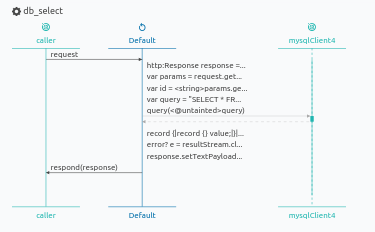
\includegraphics[scale=0.7]{figures/diagram_view_db_call.png}
	\end{center}
	\caption{Sequence diagram representation of code}
	\label{diagram_view_ballerina_code}
\end{figure}
 
It is clear that we can use the network awareness properties of the Ballerina language to identify
performance critical features directly from source code unlike other languages. Examples of network
awareness features are creating RESTful clients and servers ,making database queries , completing
asynchronous calls ,producing and consuming streaming data message-passing etc \cite{ballerina_book}.


\subsection{Thread pool tuning}

Thread pools are very important component when implementing server architectures. In SEDA every stage has its own thread pool. Creating and destroying a thread is resource intensive task for the OS \cite{thread_pool_analysis}. Instead of creating and destroying threads on demand, thread pool reuses the allocated number of threads. Size of the thread pool is almost fixed, although there are many studies to predict the number of threads in the pool dynamically using various approaches in order to gain the performance. Some approaches propose analytical models and schemes \cite{xu2004performance,thread_pool_analysis,math_aproach_thread_pool_tuning,syer2011identifying,linfeng2017design} and other approaches use run-time information \cite{lorenzon2016investigating,nieplocha2007evaluating,agrawal2006adaptive} to predict size of the pool. Most server implementation decide the number of thread in the pool heuristically and based on empirical knowledge \cite{thread_pool_analysis,math_aproach_thread_pool_tuning} to get balanced performance for every type of operations including IO since integrating analytical modeling is complex and calculation of run-time information can add an overhead to the server.

When discussing some heuristic and experience based approaches to decide the thread pool size, one rule is that the size of thread pool should be two times of the number of CPUs (processors). Ballerina scheduler is also following this rule. Another rule, used by Microsoft's IIS, initially allocates 10 threads in the thread pool per CPU, and allows the size of the thread pool to increase based on the number of client requests \cite{thread_pool_analysis}. The thread pool's maximum size is heuristically set to be two times of the number of megabytes of RAM in the host machine. Those heuristics are based on memory and CPU capabilities and there is no theoretical justification.

\textit{Yibei Ling} et al. \cite{thread_pool_analysis} propose a mathematical model to predict optimal thread pool size  by calculating cost of spawning, destroying and maintaining threads in a thread pool. However, this approach has some flaws because of assumptions they initially made. First assumption is that each thread in the pool has the same execution priority and receive uniform treatment. This is not always true because OS has limited number of processors and there are other OS level processes also using those resources. Typical modern web servers are deployed with resource control and monitoring tools as well. Thus threads may not get equal access to CPUs. The next assumption is one web request is very much like another  and that the memory and I/O resources required by different threads are minimal. This research's major focus is to optimize the sever architectures for different types of programming features specially IO. 

D.L. Freire et al.\cite{math_aproach_thread_pool_tuning} also did a similar study to calculate expected gain of web servers under different thread pool sizes using a analytical model. The optimal size of the pool depends on cost of creating threads,the cost of maintenance of the pool and the workload of the system as a probability density function. The workload can be think as the rate of receiving the client request to the web server. Experiments were evaluated under fore different  probability density function which are uniform,exponential,density of Pareto and gamma density. Then optimal thread pool size is decided for each density function. However, this study has similler assumption of above study. 
 
There are a number of parameters that can be tuned in a thread pool such as number of threads in the pool, maximum number of threads allowed in a pool, maximum time interval that a thread will be idle waiting for a new task \cite{math_aproach_thread_pool_tuning}. However most of the studies are focused only to tune the size of thread pool size since that parameter affect most when evaluating the performance of web servers. 

\subsection{The IO and Programming}

In early days one major reason to use blocking code (synchronous programming) is that it is easy to write
the program. The programmer always knows the order of code which is executing. When there is a blocking IO call ,in most cases, the wait is not really a problem because the program can not perform anything else until the I/O is finished. However, in cases such as network programming with multiple
clients, the program may wish to perform other activity as it continues to wait for more concurrent
users.
One solution for these situations is to use multiple threads so that one part of the program is not
waiting for unrelated IO to complete. But having many threads add large overhead to memory and
CPU ( thread creation and context switching is costly)
Another alternative is to use asynchronous programming techniques with non-blocking system calls.
An asynchronous call returns immediately, without waiting for the IO to complete. The completion of
the IO is later communicated to the application either through the setting of some variable in the application or through the triggering of a signal or call-back routine that is executed outside the linear
control flow of the application.
New programming languages and patterns have been adopted for exponential growth of web service
requirements and rapid development. But utilizing the program to use it’s full potential and use
resources efficiently is still a problem. Developers or programmers need to put more effort into
optimizing the programs.
One such optimization way is to write clever codes to use the blocking or waiting time on CPU for
other tasks. In order to do that, programmers need to know where the IO calls happen. But using many
libraries and knowing where the IO calls happen is a very complex task. Even though it could be
found such calls optimizing is still hard.







